\documentclass[journal]{IEEEtran}%
\usepackage[utf8]{inputenc}

\usepackage{graphicx}%
\usepackage[caption=false,font=footnotesize]{subfig}%
\usepackage{xcolor}%
\newcommand{\toDo}[1]{\textcolor{red}{#1}}%

\begin{document}
	\title{A Finite State Machine Controller for the Simulated Car Racing Championship}

\author{\IEEEauthorblockN{Bruno H. F. Macedo\IEEEauthorrefmark{1},
		Gabriel F. P. Araujo\IEEEauthorrefmark{1},
		Gabriel S. Silva\IEEEauthorrefmark{1},\\
		Matheus C. Crestani\IEEEauthorrefmark{1},
		Yuri B. Galli\IEEEauthorrefmark{1} and
		Guilherme N. Ramos\IEEEauthorrefmark{1}\IEEEauthorrefmark{2}\\[0.2cm]}
	\IEEEauthorblockA{\IEEEauthorrefmark{1}University of Brasília}
	\IEEEauthorblockA{\IEEEauthorrefmark{2}gnramos@unb.br}}

% The paper headers
%\markboth{Postgraduate Program Workshop in Computer Science}%
%{}%
%Provide better translation%
%\markboth{Workshop do Programa de P\'{o}s-Gradua\c{c}\~{a}o em Inform\'{a}tica - WPOS 2014}%
%{}%

% make the title area
\maketitle

% As a general rule, do not put math, special symbols or citations
% in the abstract or keywords.
\begin{abstract}
Electronic games can simulate extremely complex situations and be used for benchmark tests for specialized software. 
TORCS simulates a very realistic environment, and is ideal for comparing for autonomous car controllers and, consequently, the machine learning techniques applied in generating such controllers. This paper presents an AI approach to efficiently generating a car controller based on a finite state machine. Experimental results show how the controller's parameters are selected and their effect on its performance.
\end{abstract}

% Note that keywords are not normally used for peerreview papers.
\begin{IEEEkeywords}
finite state machines, computer games, Simulated Car Racing Championship, artificial intelligence
\end{IEEEkeywords}%

\section{Introduction}\label{sec:intro}
\IEEEPARstart{D}{igital} games provide a great test bed for experimentation and 
study of Artificial Intelligence (AI), and there has been a growing interest in 
applying AI in them, regardless of genre~\cite{simon2008}. Some applications 
include controlling non-playable characters~\cite{stanley2005}, path planning 
\cite{freitas2012}, human pose recognition~\cite{shotton2011}, and others. 

Electronic games also present a well defined environment, which may simulate 
extremely complex situations such as flying an airplane or controlling a car. One such simulator is \emph{The Open Racing Car Simulator} (TORCS)~\cite{TORCS}, whose input and output are constrained by the software's characteristics, providing an ideal benchmark for comparing AI solutions for creating car controllers.

Due to  the complexity of the task, most solutions attempt to develop an efficient
controller by evolving it completely, that is, by considering its performance on
the whole track. This is a very complex task, and in an attempt to
reduce this complexity, this works proposes the FSMDriver, a finite state machine 
based controller that divides the track into different types of stretches and 
evolves a state for handling each one.

The practical applications of such controllers in autonomous vehicles are enormous, 
and have been the subject of intense research for some years. For example, the 
DARPA\footnote{http://www.darpa.mil} has offered substantial prizes to winners of 
robotic challenges, the most famous being the Grand Challenge race won by Thrun 
et al.~\cite{Thrun06} .

This paper is organized as follows: Section \ref{sec:background} presents the details on TORCS and 
the Simulated Car Racing Championship and some background on finite state machines,
Section \ref{sec:fsm} describes the implementation of the FSMDriver, Section \ref{sec:results} presents 
initial experimental results, and Section \ref{sec:conclusions} provides concluding remarks.
%
\section{Background}\label{sec:background}

The Simulated Car Racing Championship (SCR) is a well-known event comprising 
three sequential competitions held in association with \textit{IEEE}, and 
present in well known conferences such as the \textit{Congress on Evolutionary 
Computation} (CEC), \textit{ACM Genetic and Evolutionary Computational Conference} 
(GECCO) and the \textit{Symposium on Computational Intelligence and Games} 
(CIG)~\cite{scr2009}.  It provides an opportunity for the scientific community 
to perform a straightforward comparison among different approaches in complex 
environments containing multiple continuous variables~\cite{caldeira_2013}. For 
this, it uses \emph{The Open Car Racing Simulator}, a state-of-the art car simulator. 

\subsection{The Open Car Racing Simulator}
TORCS provides a very customizable environment, sophisticated 3D graphics, and -
most importantly - a powerful physics simulation platform~\cite{manual}. Its 
physics engine considers static and dynamic aspects, such as fuel usage, damage 
received, wheel traction, and others, in a very detailed way. Thus, it enables 
a very complex environment for testing AI techniques.

TORCS serves both as a research platform for AI on racing development and as an 
ordinary car racing game. The main reason why TORCS is widespread in the AI gaming 
universe is its portability; it runs on all \textit{Linux}'s architectures,
\textit{FreeBSD}, \textit{OpenSolaris}, \textit{MacOSX} and both 32 and 64 bits 
\textit{Windows}. TORCS has its own online community, which started its own 
racing competitions some years ago~\cite{TORCS}, where developers can submit 
their controllers to compete with each other.The simulator's version used at the present work is torcs 1.3.4.

\subsection{The Simulated Car Racing Championship}
The SCR contest provides a standard measure for TORCS controllers by defining strict
rules, based on the Formula 1 score system~\cite{scr2009}. It improves on the 
practical applications aspects by limiting the controller's knowledge of 
the system to the information provided by its inputs and its actions by its outputs,
much like an actual autonomous vehicle.

The interface provides with a diversified set of sensors, such as the current 
position of the car in the track, its acceleration and brake values, and so on~\cite{scr2009}. 
The information provided by them defines the controllers perception of its environment (track, other controllers, etc.), and the idea is to program a behavior that results
in the best possible race. 

\subsection{SCR Contestants}
Works submitted to SCR have a wide range of variety, going from sophisticated 
heuristic designs to completely mathematical and statistical approaches. The 
controller that won the 2009 Simulated Car Racing Championship,~\cite{scr2009}
perhaps one of the most important editions realized so far, was created by 
Onieva et al.~\cite{onieva_2009}, and it 
consists of a simple set of controllers in an \emph{modular configuration}. 

Although this controller won the competition, the authors noted that it evolved 
into a fairly complex model and noted that a modular approach considerably reduce 
the effort to implement a  controller. Refactoring and debugging such a complex 
architecture requires changing code that is not directly related to the desired
change in behavior.

Another interesting controller used  artificial neural networks~\cite{cardamone_2010},
a more general approach which required little domain knowledge and provided a 
satisfactory result. Also in this case,  the implementation is quite complex and 
the final result manages connections between all inputs and outputs.

In order to reduce the effort in developing a controller, a more modular approach,
such as a \emph{finite state machine}, is desirable.

\subsection{Finite State Machines}\label{sec:fsm}

A \emph{Finite State Machines} (FSM) designates the model of a device, which has 
a finite number of states it can be in at a given moment, and which and can 
operate on input to either transition from one state to another or to cause an 
output to take place~\cite{buckland2005}. The machine can only be in one of these 
states at a given time.

FSMs have been widely used in AI applications in games~\cite{millington_2009}, due 
its inherent characteristics:

\begin{itemize}
	\item \textbf{Simplicity}: this model can be quickly implemented in many ways.
	
	\item \textbf{Flexibility}: new states can be easily incorporated into the model.
	
	\item \textbf{Modularity}: states can be independently developed in parallel.
	
	\item \textbf{Focused debugging}: since FSMs can only be in one state at a time,
	debugging/testing is limited to the state in question.
	
	\item \textbf{Small computational overhead}: states are usually implemented 
	with hard-coded rules concerning a specific situation, which in turn demands
	small amounts of processor time.
	
	\item \textbf{Intuitive behavior}: analyzing a FSM is an easy process for 
	humans because we are always intuitively categorizing situations and behaviors,
	just like a FSM working. 
\end{itemize}
%
\section{The FSM Driver}\label{sec:fsm}
The proposal for controlling the car is a \emph{Finite State Machine}, which
enables a modular development, ideal for teamwork, and separates behaviors, reducing
the effort necessary to evolve a complete controller by breaking this problem into
evolving each state.

From the intuitive perspective of a human driver in a car race competition, there 
is a clearly defined desirable behavior: to \emph{drive faster than the competitors}.
The simulation account for different environment conditions, therefore a car's 
performance is always better, everything else being the same, when it is within 
track limits than outside. So this rather complex behavior which can be broken into specific behaviors: \emph{drive as fast as possible on the track} and, 
in case something goes wrong, \emph{get back on the track as fast as possible}.

Driving as fast as possible on a straight line is simple, but a different behavior
than doing it in a curve, thus the state can be further divided into \emph{drive
drive as fast as possible in a straight line} and \emph{make the
curve as fast as possible}. Finally, because racing usually implies being able to
move forward, a behavior for handling situations when that is not possible is 
necessary.

\begin{figure}
	\centering
	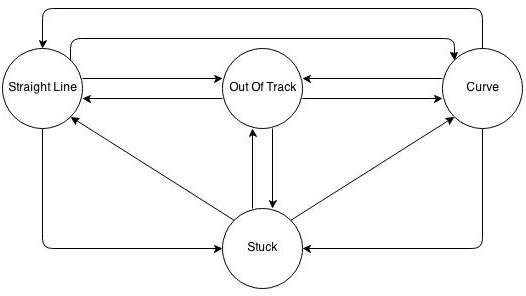
\includegraphics[width=3in]{StatesDiagram}
	\caption{State transition diagram.}
	\label{fig:fsm}
\end{figure}

Therefore, FSMDriver's initial configuration has four states, as illustrated in 
Fig. \ref{fig:fsm}, described as follows: 

\begin{itemize}
	\item \textbf{Straight Line}: the controller commands the car to full throttle 
	with maximum acceleration straight ahead, adjusting the steering to stay in 
	the middle of the track.
	
	\item \textbf{Curve}: the controller handles curves based on the position of 
	the car and the angle between the direction of the axes of the car and the 
	track axis, adjusting the steering, gear, and clutch actuators to keep it 
	moving as fast as possible within track limits while trying to avoid damage
	(by crashing into another car or wall).
	
	\item \textbf{Out of Track}: the controller tries to return to the 
	track as fast as possible by steering in an arbitrary angle (with 
	relation to the track's axis of track). Due to low friction outside of the 
	track, accelerating and braking are proportional to the sideway speed of the 
	car to minimize skidding.
	
	\item \textbf{Stuck}: the controller takes drastic measures to try to recover, 
	using reverse gear and hard steering to try to get back on track in this worst 
	case scenario.
\end{itemize}

There are two states for usual on track regular on track situations and two for
off track ones. Only one of these states will be in control at a time, but all 
have to work together to handle the all possible scenarios and each has to be
properly configured to achieve competitive results.

The complete behavior is achieved by transitioning between states, this is 
implemented in a \texttt{transition} function that uses specific parameters to decide when 
the current state needs to be changed (and which state to change to). This function 
operates on four constant parameters:
	\begin{itemize}
		\item[$MSD$,] the maximum speed distance, which defines the 
		maximum value for the frontal sensor input while racing at full speed;
		\item[$LE$,] the track's left edge boundary, which defines the area
		available for moving the car left;
		\item[$RE$,] the track's right edge boundary, which defines the area
		available for moving the car right;
		\item[$ST$,] the number of stuck ticks, required by the controller 
		for identifying how long it has not been moving fast enough and, thus,
		concluding it is stuck.
	\end{itemize}

\texttt{transition} analyses the car's inputs to define if there has to be a
change in state on every simulation tick. The first procedure is to check if the
car is \textbf{Stuck}, that is, if it is has a very low speed (obviously, ignoring 
the beginning of the race when all cars ares stopped), then a counter is incremented 
and its value compared to the $ST$ threshold.

In case the car is not stuck, \texttt{transition} will define the current state
by analyzing its position in the track. It will be \textbf{Out of Track} if it is
out of the range defined by $LE$ and $RE$. Otherwise, it is considered 
on track and can be either on a \textbf{Straight Line}, if the frontal distance 
sensor's input is larger than $MSD$ or when it is larger than the input of the 
adjacent side sensors, or on a \textbf{Curve} otherwise. %
\section{Experimental Results}\label{sec:results}
For initial evaluation of FSMDriver, only changes in the transition function's 
parameters were tested, with a simple iteration over arbitrary values for all. At
each iteration, only one parameter value was changed. Table \ref{tbl:parameters} shows the parameters, their initial ($V_I$) and final 
($V_F$) values, and the step ($\Delta$) taken in each iteration. 

\begin{table}[h]
\renewcommand{\arraystretch}{1.3}
\caption{Transition Parameters}
\label{tbl:parameters}
\centering
\begin{tabular}{c||c||c||c}
\hline \bfseries &\bfseries $V_I$ &\bfseries $V_F$ &\bfseries $\Delta$ \\
\hline
\hline MSD & $20$ & $200$ & $5$ \\ 
\hline LE & $-1$ & $-0.8$ & $0.1$ \\ 
\hline RE & $0.8$ & $1$ & $0.1$ \\ 
\hline ST & $30$ & $300$ & $10$ \\ 
\hline 
\end{tabular} 
\end{table}

For each of the over 8500 configurations, experiments consisted of 3 laps, in 
the B-Speedway and CG-Speedway 1 tracks (see Fig. \ref{fig:tracks}), each race 
starting with one car fully stopped. B-Speedway provides the simplest track for 
validation, while CG-Speedway 1 has more characteristics of usual race tracks, 
such as sharp curves for either side, and provides a more general idea of the 
FSMDriver's behavior.

\begin{figure}
\centering 
\subfloat[B-Speedway]{
\includegraphics[width=1.2in]{B-Speedway}}
% \label{fig_first_case}} 
\hfill
\subfloat[CG-Speedway]{
\includegraphics[width=1.2in]{CG-Speedway}}
% \label{fig_second_case}} 
\caption{FSMDriver test tracks.} 
\label{fig:tracks} 
\end{figure} 

Results are evaluated by total race time, smaller being better. The parameter values 
for the fastest races are presented in Table \ref{tbl:best_config}.
It is interesting to note that many configurations yielded the same results, and 
that \textbf{Straigh Line}'s steering control is sufficient for it to run on wide
curves, there no transitions were triggered in B-Speedway's tests.

\begin{table}[h]
% \renewcommand{\arraystretch}{1.3}
\caption{Best Configuration}
\label{tbl:best_config}
\centering
\begin{tabular}{c||c||c||c||c}
\hline & MSD & LE & RE & ST \\ \hline\hline
B-Speedway & 20 & -0.8 & 1 & 110 \\\hline
CG-Speedway 1 & 20 & -0.8 & 1 & 110 \\\hline
\end{tabular} 
\end{table}

To further analyze FSMDriver's behavior, it is  
compared to default controllers provided by the TORCS distribution. One of the 
maintainers of TORCS, Bernhard Wymann\footnote{www.berniw.org}, has created
a wide range of controllers with diverse characteristics, from average racing 
behavior like \emph{berniw3} to one of the best controllers available \emph{berniw1}.
In this test, controllers had a 3 lap race (by themselves) and total time was 
evaluated. Results are shown in Tables \ref{tbl:berniw_B} and \ref{tbl:berniw_CG}.

\begin{table}[h]
\renewcommand{\arraystretch}{1.3}
\caption{3 Laps in B-Speedway}
\label{tbl:berniw_B}
\centering
\begin{tabular}{c||c||c||c}
\hline
\bfseries Driver & \bfseries Total Time & \bfseries Damage & \bfseries Top Speed \\ 
\hline
\hline Berniw 1 & 02:25:65 & 6 & 321 \\
\hline Berniw 2 & 02:25:65 & 6 & 321 \\
\hline Berniw 7 & 02:27:20 & 0 & 308 \\
\hline Berniw 6 & 02:27:46 & 0 & 309 \\
\hline Berniw 8 & 02:27:75 & 0 & 307 \\
\hline Berniw 9 & 02:28:10 & 0 & 306 \\
\hline Berniw 5 & 02:28:58 & 2 & 307 \\
\hline Berniw 4 & 02:29:42 & 3 & 303 \\
\hline Berniw 3 & 02:31:38 & 0 & 301 \\
\hline FSMDriver & 02:34:95 & 1 & 299 \\ 
\hline Berniw 10 & 02:40:70 & 8 & 282 \\ 
\hline 
\end{tabular}
\end{table}

\begin{table}[h]
\renewcommand{\arraystretch}{1.3}
\caption{ 3 Laps in CG Speedway 1}
\label{tbl:berniw_CG}
\centering

\begin{tabular}{c||c||c||c}
\hline \bfseries Driver &\bfseries Total Time &\bfseries Damage &\bfseries Top Speed \\
\hline
\hline Berniw 8 & 02:07:17 & 0 & 246 \\
\hline Berniw 6 & 02:07:18 & 0 & 248 \\
\hline Berniw 4 & 02:07:18 & 0 & 246 \\
\hline Berniw 7 & 02:07:20 & 0 & 250 \\
\hline Berniw 5 & 02:07:28 & 0 & 246 \\
\hline Berniw 3 & 02:07:28 & 0 & 247 \\
\hline Berniw 9 & 02:07:58 & 0 & 247 \\
\hline Berniw 1 & 02:12:80 & 1 & 252 \\
\hline Berniw 2 & 02:12:80 & 1 & 252 \\
\hline Berniw 10 & 02:21:54 & 0 & 230 \\
\hline FSMDriver & 02:34:49 & 3337 & 242 \\ 
\hline 
\end{tabular}
\end{table}

As expected, this initial version of FSMDriver does not have the outstanding 
behavior of \emph{berniw1}, but its results show that the proposal does have
acceptable performance, and future tweaking of FSMDriver's states parameters may
lead to better results. It is also important to note that the TORCS controllers
have a different implementation, one that has access to the simulator's inner data,
while FSMDriver's behavior is defined exclusively by its available sensors.

After analyzing FSMDriver's performance in CG-Speedway 1, it was clear from the
amount of damage that the problem was that the controller was consistently going
out of the track and hitting the wall. After further inspection, this was found 
to happen after stretches of straight lines, when FSMDriver would accelerate as 
much as possible and enter a curve going too fast for proper steering.

This indicates the need for another state, \textbf{Approaching Curve}, in which 
FSMDriver would adjust between current behaviors and enter the curve in a better
condition to make it as fast as possible.%
\section{Conclusion and Future Works}\label{sec:conclusions}
Digital games provide an excellent opportunity to experiment and study the 
different applications of Artificial Intelligence, such as controlling an autonomous
vehicle. The The Simulated Car Racing Championship is used as a standard test for 
such controllers, allowing different solutions compared in a straightforward manner.

This work presents the early stages of FSMDriver, a finite state machine approach
to developing a controller. The goal is to eventually compete in SCR by improving
the controller's behavior though machine learning techniques. This first version
considers four states for defining its racing behavior: \textbf{Straight Line}, 
\textbf{Curve}, \textbf{Out of Track}, and \textbf{Stuck}. Overall, the results
obtained in this world provided very valuable information to guide future 
developments of the proposal.

Initial experimental results showed that the approach is feasible, as FSMDriver
can successfully complete races and even be faster than some of the available
TORCS controllers. They also showed that adjusting configuration parameters lead 
to improved behavior, further efforts using machine learning techniques to 
improve this are being pursued.

Comparison to existing controllers showed that FDSMDriver's first version has 
average behavior, and there is much work to be done. To this end, future versions
will consider not only the parameters that define transitions between states, but
also the states' internal parameters.

Analysis of race conditions indicated an immediate need for a new state to handle 
between a straight stretch of track and a curve. Because experimental results 
showed extreme damage to the car due to crashing to the wall, it is likely that 
a state to \emph{avoid collisions} will be necessary. This could also be used to 
handle adversary cars.%

\bibliographystyle{IEEEtran}%
\bibliography{bibliografia}%

\end{document}
